\chapter{Functional programming} 
\vspace{-1cm}
Functional programming is a programming paradigm 
to mimic mathematical functions. 
It can be considered a declarative programming language 
that builds complex functions by functional composition. 
Functional Programming is based on Lambda Calculus developed 
by Alonzo Church (1903-1995). 
Alan Turing (1912-1954), who was a student of Alonzo Church, created the 
universal Turing machine which laid the foundation of imperative 
programming style.
In 1957, Fortran language was created by John Backus(1924-2007).
In 1977, Backus described the Function Programming (FP) in his famous Turing Award lecture:
 "Can Programming Be Liberated from the von Neumann Style?".
%In the mid 1980s Backus and his colleagues came up with the language FL. 
%Python and Fortran both support functional programming in some degree.  
In this chapter, the following concepts, associated to functional 
programming paradigm, will be discussed through  different examples 
for Python and Fortran:  
\vspace{-0.25cm}
\begin{enumerate} 
 \setlength\itemsep{0cm}
\item First-Class functions.
\item Pure functions and side effects.
\item Recursion. 
\item Map, filter and reduce elemental functions.  
\item Modularity. 
%\item Closure.
\item Referential transparency. 
\end{enumerate} 
\vspace{-0.25cm}
Main advantages of functional programming are: its closeness 
to mathematical formulation, its ability to avoid side effects and 
its modularity to partition complex problems into easier ones.
One of main disadvantages is a lower  computational performance 
than imperative paradigm associated to recursion and functional composition
techniques.  Functional programming is usually used in mathematical 
computations and when parallelism or concurrency is required.


 
\newpage
 \section{First-class functions} 
A programming language has first-class functions 
when functions can be treated like any other variable. 
Namely, functions can be used in the following situations:  
\begin{enumerate} 
\item Function with arguments that are also functions.
\item Functions returning functions. 
\item Functions being assigned to other functions.
\end{enumerate} 

\subsection{Functions as arguments} 
Many mathematical concepts or functions are defined for a 
specific set of functions.
For example, the integral of some function is defined by: 
\begin{equation}
 I = \int _a ^b f(x)  \ dx, \qquad f: \mathbb{R} \rightarrow \mathbb{R}
\end{equation} 
It is desirable to implement a function to determine the definite integral
in the compact segment $ [a, b ]$ for any  
$  f: \mathbb{R} \rightarrow \mathbb{R} $. 
In order to have a complete example, an approximate method is needed to 
define the integral. Let's consider the right Riemann sum 
as an approximation by a finite sum: 
\begin{equation}
 I \approx \sum _{i=1} ^N f(x_i)  \ ( x_i - x_{i-1} ),
\end{equation}
where $ x_i $ is a partition of $ [a, b]$ 
\begin{equation}
 a = x_0 < x_1  < \cdots < x_N = b.
\end{equation}
In the following scheme, the interface of function integral is defined:  

\begin{center} 
 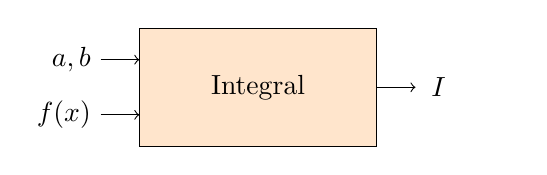
\begin{tikzpicture}
 \node[draw, fill=orange!20, minimum height=1.5cm, minimum width=3cm] (node) at (0,0) {Integral};
 \draw[->] (-2,0.35)node[anchor=east] {$a,b$} to (\tikztostart -| node.west);
 \draw[->, black] (-2,-0.35) node[anchor=east] {$f(x)$} to (\tikztostart -| node.west);
 \draw[->]  (1.5,0) node  {} to (2,0);
 \node[text width=1cm] at (2.7,0) {$I$};
 \end{tikzpicture}
\end{center} 



  
 \newpage 
  \subsubsection*{Fortran} 
The main purpose is to write a function with three arguments. The two first
are real numbers: $ a $ and $ b$. 
The interface definition of third argument  
$( f: \mathbb{R} \rightarrow \mathbb{R} ) $
is expressed with the following code:  
\vspace{0.5cm} 
   \renewcommand{\home}{./Fortran/sources/Advanced_programming/functional programming} 
   \lstfor
  \listings{\home/First_class_functions.f90}{abstract interface}
  {end interface}{First_class_functions.f90}
Once every argument is defined, the function integral is implemented: 
%  \listings{\home/First_class_functions.f90}{subroutine Function_examples}
%  {end subroutine}{First_class_functions.f90}
 \vspace{0.3cm}  
 % \newpage 
  \listings{\home/First_class_functions.f90}{real function Integral}
  {end function}{First_class_functions.f90}
Note that the third argument is a procedure function defined above. 
The following example creates a function $ h(x) $ to be integrated 
using the new function \verb|Integral|. 
 \vspace{0.3cm}  
  \listings{\home/First_class_functions.f90}{real function h}
   {end function}{First_class_functions.f90}
 
\newpage
\subsubsection*{Python}
Since Python is untyped language, 
\verb|Integral| function is implemented without specifying the type of its
arguments with the following code: 
\renewcommand{\home}{./Python/sources/Advanced_programming/functional programming}
\lstpython 
\vspace{0.5cm}
\listingsp{\home/First_class_functions.py}{def Integral}
  {return}{First_class_functions.py}
Note that the extension of the \verb|Integral| function has been reduced 
drastically by sacrificing 
the specifications or variables and arguments. 
Once someone makes use of this function, the Python interpreter will 
check dynamically that the operations involved in the above code 
are defined.
If the function $ h(x) $ is defined by: 
\vspace{0.5cm}
\listingsp{\home/First_class_functions.py}{def h}
  {return}{First_class_functions.py}
by invoking 
\vspace{0.5cm}
\listingsp{\home/First_class_functions.py}{R = Integral}
  {print}{First_class_functions.py}
will work without any problem.    

\newpage 
\subsection{Functions returning functions} 
In mathematics, 
function composition is an operation 
that takes two functions $f$ and $g$, and yields a function $ h = g  \circ  f  $ 
such that $ h(x) = g(f(x))$. 
Once the image of $ x $ is obtained by applying the function $ f $, 
a new image  $g(f(x))$ is yielded by applying $ g $. 

In Fortran language, functions can not return functions. 
The only possibility is to create derived types comprising 
functions or procedure pointers. This strategy is closer to the
Object Oriented Programming and it will treated in next chapters. 
However, Python allows very intuitively to build functions returning functions. 

\subsubsection*{Python}
The following example shows the definition of a function which returns 
the function composition of $ f $ and $ g $
\lstpython 
\vspace{0.5cm}
\listingsp{\home/First_class_functions.py}{def compose}
  {return h}{First_class_functions.py}
  
\subsection{Functions being assigned to other functions} 
Following with the same mathematical example, 
the creation of a new composition function is written in mathematical 
language as:
\begin{equation}
     h = f \circ g  
\end{equation} 
Fortran does not allow to assign functions to each other. 
The same strategy described above based on function or procedure pointer can be used to 
overcome this deficiency. However, Python allows to assign function
 as if they were variables as it is shown in the following code snippet: 
\lstpython 
\vspace{0.4cm}
\listingsp{\home/First_class_functions.py}{sqrt}
  {sqrt}{First_class_functions.py}




\newpage   
\section{Pure functions} 
In computer programming, a pure function is a function 
that returns values identical for identical arguments
and has no side effects. 
Hence, a pure function is a computational analogue of a mathematical function. 
Pure functions can be explicitly declared in Fortran with the \verb|pure| attribute.
However, in Python there is no way to force a function to be pure.  
The following list constitutes the requirements for a function to be pure.    
 \begin{enumerate}
  \setlength\itemsep{0.1cm}
 \item The function must not alter any dummy argument. 
 To accomplish that in Fortran,  arguments must have \verb|intent(in)| attribute 
 unless they are procedures or pointers.   
 \item The function must  not alter any part of a variable accessed by host or 
 use association. 
 \item Local variables can not have the \verb|SAVE| attribute(Fortran) or be saved. 
 \item Functions as arguments must be pure. 
 \item No external input/outputs operations are allowed. 
 \item STOP is not allowed. 
 \end{enumerate}   
If the Fortran function is declared with the \verb|pure| attribute and any of those 
requirements are not fulfilled, the compilation process of the source code will prompt an error.
In Python if pure functions are required, special care should be taken into account with these 
requirements. 
Those requirements are needed to assure that pure functions returns 
the same values for identical input arguments. 
One of main characteristics of any software development strategy is data hiding. It means that
non necessary data should be hidden to avoid bugs or improper behavior. 
However, when external data or global variables are needed, 
pure functions must not modify those variables. 

It seems that writing the entire code with pure functions would be our goal to improve 
efficiency in developing software. However, sometimes because a database should be modified 
or a random number generator is used, the same output is not obtained. 
The goal is to use pure functions when practical. Total purity 
is not practical but what about  80\% purity.


For sake of clarity, requirements to implement pure functions are  discussed in the following example: 
\newpage  
    \renewcommand{\home}{./Fortran/sources/Advanced_programming/functional programming} 
    \lstfor
   \listings{\home/First_class_functions.f90}{pure_functions}
   {end subroutine}{First_class_functions.f90}
The function \verb|f(x)| is declared to be pure. It has only one argument a real value \verb|x|.
As it was mentioned, \verb|x| must be specified with the \verb|intent(in)| attribute 
in order not to be modified accidentally.
A local variable \verb|b| is declared. This local variable can not have the \verb|SAVE| attribute
or can not be initialized to avoid undesirable historical effects. 
The function \verb|f_impure(x)| is impure because it has the initialization \verb|real::b=1|.
The first time this function is called with $ x=1$, it gives \verb|4,0| and the second time 
it yields \verb|5.0|. The reason is because the variable \verb|b| is only initialized at compilation 
time and saved for future calls. The first time \verb|f_impure(x)| is called, 
and after the sentence \verb|b=b+1|, variable \verb|b| holds \verb|2.0|. 
The second time \verb|f_impure(x)| is called, 
and after the sentence \verb|b=b+1|, variable \verb|b| holds \verb|3.0| and 
 \verb|f_impure(x)| gives a different value than the first call with identical input \verb|x|. 
Those are typical errors that can be avoided by writing  pure functions.

   


\newpage  
\section{Recursion}
\vspace{-0.5cm}  
In mathematics, a recursive definition or inductive definition, 
is used to define the elements in a set in terms of other elements in the set.
A recursive function is a function that its value at any point can be calculated 
from the values of the function at some previous points. 
For example,  the Fibonacci sequence 
\begin{equation} 
F(n) = F(n-1) + F(n-2)
\label{Fibonacci} 
\end{equation}
gives $ F(n) $ once $ F(n-1) $ and $F(n-2)$ are known. If the function values at  $n=0$  and 
$ n=1$ are known, the function value at $ n=2$ can be obtained from  the equation (\ref{Fibonacci}).
Recursive functions in programming languages allows to obtain the sequence 
from the declarative point of view. That is, it is not need to develop an iterative 
or imperative procedure as it is described above. 
As it was mentioned, recursive procedures are less efficient in terms of computational 
resources than iterative implementations. However, recursive implementations are easier to 
debug and to implement.  
 
\vspace{-0.5cm}
\subsection*{Fortran}
 \renewcommand{\home}{./Fortran/sources/Advanced_programming/functional programming} 
    \lstfor
   \listings{\home/First_class_functions.f90}{function Fibonacci}
   {end function}{First_class_functions.f90}
   \vspace{-0.8cm}
\subsection*{Python}
 \renewcommand{\home}{./Python/sources/Advanced_programming/functional programming} 
    \lstpython
   \listingsp{\home/First_class_functions.py}{def Fibonacci}
   {n-2}{First_class_functions.py}
   
   
 
  
\newpage  
\section{Map, filter and reduce}

In mathematics, mapping refers to the action of applying a function to the elements of its domain.
Mapping applies to any set: a collection of objects. 
\begin{equation} 
   f:A \rightarrow B 
\end{equation}    
is a map from $ A $ to $ B$; for every 
$ a $  in $ A$, there is a unique object $ f(a)$  in $ B$.
For example, rotating 
a body about a point is a map that transforms the body coordinates into new coordinates 
keeping the axes fixed. 



A filter tests each element of a set with a unary predicate. 
Elements that satisfy the predicate are kept and  those that don’t are removed. 
A filter on a set $ X $ is 
a subset  $ B \subseteq X $.


Reduce combines the elements of the set together using a binary function to get a scalar result. 
Examples of functions that perform reduction on arrays are: sum, product, all, any, minval,  maxval, maxloc
and minloc.



 
 


\vspace{1cm} 
\begin{IN}
The mathematical concepts: map/filter/reduce allow a software design 
simplifying the implementation of functions that operate over sequences of elements
enabling an implementation with no explicit control flow, not a single loop or if statements.
\end{IN}
\vspace{0.5cm} 
These mathematical concepts are taken into account in a functional programming language 
such as Python and Fortran and they will be explained in the following sections through examples.







\newpage 
\subsection{Mapping} 
To explain the implementation of the map functionality, let's consider a rotation 
which is a map of a plane into itself. The rotated coordinates of the point $(x,y)$ with an angle 
$\theta$ are: 
\begin{equation}
\begin{pmatrix}
x_r \\
y_r
\end{pmatrix}
=
\begin{pmatrix}
cos \ \theta & -sin \ \theta\\
sin \ \theta &  cos \ \theta
\end{pmatrix}
\begin{pmatrix}
x \\
y
\end{pmatrix}
\label{rotation} 
\end{equation} 
In the following example a square is rotated $ \pi/4 $ radians.
\subsubsection*{Fortran}
\renewcommand{\home}{./Fortran/sources/Advanced_programming/functional programming} 
  \lstfor
 \listings{\home/map_filter_reduce.f90}{type :: point2D}
 {end type}{map_filter_reduce.f90}
 \listings{\home/map_filter_reduce.f90}{function Rotation}
  {end function}{map_filter_reduce.f90}
\listings{\home/map_filter_reduce.f90}{image =}
  {imageR =}{map_filter_reduce.f90}  
First, the new type \verb|point2D| is defined. It is determined by its $ (x,y)$ coordinates. 
Then, rotation equation (\ref{rotation}) is implemented in \verb|Rotation|.
Finally, a set of  \verb|point2D| points is mapped with the \verb|Rotation| function which is written 
for a generic \verb|point2D| point. Note that the attribute \verb|elemental| of this function allows
to apply this functions for isolated elements or for a whole set of points. 

\subsubsection*{Python}
\renewcommand{\home}{./Python/sources/Advanced_programming/functional programming}
 \lstpython
 \listingsp{\home/map_filter_reduce.py}{def Rotation}
  {return}{map_filter_reduce.py}
  \vspace{0.5cm} 
\listingsp{\home/map_filter_reduce.py}{image =}
  {imageR =}{map_filter_reduce.py}  
Since Python is an untyped langauage, there is no need to define the plane point \verb|P|.
Hence,  \verb|Rotation| function is implemented assuming that \verb|P| is an numpy array with 
two components. This is assumed from expression \verb|matmul(A, P)|. 
Since \verb|A| is a square matrix of dimension 2, \verb|P| should be a vector of dimension 2 
 to have a conformal operation. 
 
Finally, a set of points is mapped with the \verb|Rotation| function which is written 
for a generic point. Note that the keyword \verb|map| allows this mapping. 
The first argument of \verb|map| is the scalar function to be applied to each element 
of the set and the second argument is the set. Since \verb|Rotation| has two arguments: 
point and angle to be rotated, a \verb|lambda| function is used to define a 
new function with only one argument.  



  
  
 \newpage 
\subsection{Filter and reduce} 
In Fortran, filtering is accomplishing by the intrinsic function \verb|pack| and
reduce operation with different functions. In this example, \verb|minloc| is used.   
A set of random two dimensional points is generated 
in the square $ [-1, 1] \times [-1,1]$.  This set of points is filtered through the \verb|filter|
function which determines if the point is inside the region enclosed between
the two concentric circles of radius \verb|R1| and \verb|R2|. Since the function \verb|filter|
has \verb|elemental| attribute, the statement \verb|filter(set, 0.4, 0.7)| constitutes 
a mapping for all elements of \verb|set|. The intrinsic function \verb|pack|
filters the complete \verb|set| yielding a \verb|subset|. Finally, \verb|minloc| is used 
as an example of reduce functions. 

\vspace{-0.5cm}
  \subsection*{Fortran} 
  \renewcommand{\home}{./Fortran/sources/Advanced_programming/functional programming} 
   \lstfor
  \listings{\home/map_filter_reduce.f90}{subroutine test_filter_reduce}
  {Nearest}{map_filter_reduce.f90}
   
  \listings{\home/map_filter_reduce.f90}{function filter}
  {end function}{map_filter_reduce.f90}
  
  
\newpage 
\subsection*{Python}
In Python, filtering is accomplishing by the intrinsic function \verb|filter| and
reduce operation with different functions. In this example, \verb|armin| is used.   
A set of random two dimensional points is generated 
in the square $ [-1, 1] \times [-1,1]$.  
This set of points is filtered through the \verb|filter_d|
function which determines if the point is inside the region enclosed between
the two concentric circles of radius \verb|R1| and \verb|R2|. Since the function \verb|filter_d|
has three arguments, a lambda function is used to meet the requirement of the first a argument 
of the function \verb|map|. The result of \verb|filter| is transformed a list and later to a
numpy array.  Finally, \verb|argmin| is used 
as an example of reduce functions.  
  
\vspace{0.5cm}   
  \renewcommand{\home}{./Python/sources/Advanced_programming/functional programming}
  \lstpython
  \listingsp{\home/map_filter_reduce.py}{def test_filter_reduce}
  {Nearest}{map_filter_reduce.py}
  \listingsp{\home/map_filter_reduce.py}{def filter_d}
  {return}{map_filter_reduce.py}
   \listingsp{\home/map_filter_reduce.py}{distance}
    {return}{map_filter_reduce.py}
  
  
  
 \newpage 
 \subsection*{Fortran} 
 In this last example, an array of char strings
 containing numbers  is transformed to an array numbers by means of a mapping. 
 Then, the array is filtered (\verb|pack|) retaining only those elements which are greater than 
 200 and, finally, a reduce function \verb|maxval| is used  to obtain the maximum value of the 
 array. 
 \vspace{0.5cm}
 \renewcommand{\home}{./Fortran/sources/Advanced_programming/functional programming} 
  \lstfor
 \listings{\home/map_filter_reduce.f90}{subroutine test_map_filter_reduce}
 {end subroutine}{map_filter_reduce.f90}
  \vspace{0.5cm}
 \listings{\home/map_filter_reduce.f90}{elemental integer function str_to_number}
 {end function}{map_filter_reduce.f90}
 
 
\newpage 
\subsection*{Python}
In this last example, a list  of char strings
containing numbers is transformed to a list of numbers by the \verb|map| function. 
Then, the list is filtered (\verb|filter|) with \verb|my_filter| predicate
retaining only those elements which are greater than 
200 and, finally, a reduce function \verb|max| is used to obtain the maximum value of the 
list. 
 \vspace{0.5cm}
 \renewcommand{\home}{./Python/sources/Advanced_programming/functional programming}
 \lstpython
 \listingsp{\home/map_filter_reduce.py}{def test_map_filter_reduce}
 {max value}{map_filter_reduce.py}
 \vspace{0.5cm}
 \listingsp{\home/map_filter_reduce.py}{def str_to_number}
 {return}{map_filter_reduce.py}
 \vspace{0.5cm}
 \listingsp{\home/map_filter_reduce.py}{def my_filter}
  {return}{map_filter_reduce.py}
 
 
\newpage   
\section{Modularity} 
Modular programming is a software design technique that separates 
the functionality of a program into independent modules containing 
specific aspects  of the required functionality.
Modular programming developed in the late 1960s and 1970s, 
as a larger-scale analog of the concept of structured programming (1960s).
Structured programming was developed to improve the clarity of a computer 
program by making use of the structured control flow sentences (if/then/else, while/for).
Modular programming  refers to the high-level decomposition of the code 
and structured programming refers 
to the low-level code use of structured control flow.

Python and Fortran allows to develop huge programs based on different modules.
In Python,  modules are source Python files containing functions that 
can be imported or used easily from another Python file. It can be considered a Python library. 
In Fortran, modules are specified by the name \verb|module xxx| and they can be stored in Fortran
source files. To follow the same methodology than Python, it is advisable to name that 
Fortran source file with same name  than the module storing only one module per file. This 
Fortran file \verb|contains| functions. 
Since Python is an untyped language, interface of functions is unknown when imported. 
This is a double-edge sword. The favorable consequence is the same function could be used 
for different data types if the involved operations are defined. The bad consequence is that 
errors associated to wrong use of the functions are only detected at run time. 
On the contrary, Fortran has explicit interface of all public functions contained in some module 
when it is used. This explicit interface allows to correct 
implementing errors at compiling time. However, overloading is needed when 
calling those functions with new types. 
In both languages, modularity is a pillar in functional programming creating 
abstractions in a hierarchical fashion.

For example, to solve a nonlinear system of partial differential equations, 
the following layers or modules can be defined: 
\begin{enumerate}
\setlength\itemsep{0cm}
\item Application layer: solve a nonlinear system of partial differential equation. 
\item Discretization layer: discretization method for partial differential equations.  
\item Non linear solver: functions to solve nonlinear system of equations 
such as Newton method.
\item Linear algebra:  methods to solve linear systems of equations. 
\end{enumerate}
The original complex problem is formulated by functional composition into smaller
or simpler problems or functions. 
One of the main goals of modularity in functional programming is the ability to 
build different methods of different modules without knowing the functionality of 
other modules. Besides, an extra effort must be put to define the hierarchical 
structure.  


 

 
 
  
%\newpage  
%\section{Closure} 
%
% 
% \newpage 
%  \renewcommand{\home}{./Fortran/sources/Advanced_programming/functional programming} 
%  \listings{\home/First_class_functions.f90}{real function Moment}
%  {end function}{First_class_functions.f90}
%  
%
% and lexical scoping
%
%
%Lexical scoping defines how variables are seen in nested functions.
%When functions are defined inside other functions, the scope of this inner 
%function comprises local variables of the actual function and 
%local variables of those outer or parent functions.
%
%
% 
%inner functions contain the scope 
%of parent functions even if the parent function has returned.
% 


\newpage  
\section{Referential transparency}  
In functional programming, referential transparency is defined as the fact that an 
math expression involving function evaluations can be
simplified or rewrite in different order without changing the result of the program.
The concept was originated in Alfred North Whitehead and 
Bertrand Russell's Principia Mathematica (1910–13).
Mathematical concepts, such as simplification or factorization applies also
to functional programming. Imagine, for example, the following math expression: 
\begin{equation}
g(x) + g(x) \ ( h(x) - 1 ). 
\end{equation} 
By extracting the common factor $ g(x) $, the expression simplifies to yield: 
\begin{equation}
 g(x) \  h(x). 
\end{equation} 
This is always true for mathematical functions. However, 
when trying to simplify expressions in a programming code, it is only valid when dealing 
with pure functions. 
Imagine the following example with  $ g(x) $ impure: 
 \vspace{0.5cm}
 \renewcommand{\home}{./Fortran/sources/Advanced_programming/functional programming} 
  \lstfor
  \listings{\home/First_class_functions.f90}{referential_transparency}
 {end function}{First_class_functions.f90}
Every time $ g(x) $ is evaluated, the statement \verb|b=b+1| increases by one the 
\verb|b| variable
yielding different values of $ g(x)$ for identical values of its argument $x$ 
($g(x)$ is an impure function). 
In this example, the first expressions gives \verb|3.0| and the simplified expression 
gives  \verb|5.0|. It is said tha the above expression is not referentially transparent 
and this simplification is not allowed or gives different results. 
Referential transparency is desirable property 
to factorize or simplify programming codes. 
%To attain referential transparency, all functions and procedures 
%should be pure.  
If all functions involved in some expression are pure functions, 
then the expression is referentially transparent.


\newpage
\subsection{Benefits of referential transparency} 
When developing huge numerical codes, specifications are not always perfectly clear. 
Final specifications usually evolve with results of different tests. Besides, it is very easy to 
write impure functions when external or global variables are needed.
Math abstractions are explored and defined at the same time or after the code is functional. 
Additionally,  when different developers are involved,  
similar or repetitive functions are written making grow the code unnecessarily. 
All these issues usually originate  huge codes that should be 
rewritten to yield: robust, easy to maintain, more efficient and fast codes. 
From the point of view of the authors, these issues eventually originate 
the following three categories of programming code: 
\begin{enumerate}
\item Spaghetti code. Usually, imperative programming dominates the scenario. 
\item Encapsulated code. Some effort is put in functions isolation but a real hierarchical 
 structure is missing. 
\item Multilayer code. Simple math abstractions are encapsulated in pure functions and 
more complex functions are built by function composition of pure functions. 
\end{enumerate}
The main benefit of referential transparency  is
the ability to read, understand, reason about and modify our 
functions without altering the external world. 
When the code is written with pure functions, different developers are able to write 
their pure functions without knowing the code of other programmers or other layers. 
Even if they need the outputs of some layers that are not written yet, the referential
transparency allows to substitute these functions by emulators that gives
the value it is supposed to yield. 


Functional programming  with referential transparency or pure functions allows to rewrite and reorder 
a huge programming code easier than imperative programming. 
The semantics of an imperative programming language is based on definition 
and ordering of different sequence points.
If the substitution of an expression with its value is valid only at a certain point 
in the execution of the program, then the expression is 
not referentially transparent. 
However, pure functional programming 
is referentially transparent and expressions can be evaluated at any time. 
Hence, there is no need to define sequence points and no need 
to guarantee of the order of evaluation. 
This advantage allows to test the code with compilers or to refactor
the code with intelligent tools. 

Other benefits of referential transparency is refactoring and maintenance tasks. 
Huge numerical programming codes are always evolving by including new functionalities 
or by improving theirs performances. 

  
  
  